\chapter{Vector Calculus---The Language of Change and Optimization}

\begin{quote}
    \itshape
    ``The calculus is the greatest aid we have to the appreciation of physical truth in the broadest sense of the word.''
    
    \raggedleft--- William Fogg Osgood
\end{quote}

\begin{quote}
    \itshape
    ``In mathematics you don't understand things. You just get used to them.''
    
    \raggedleft--- John von Neumann
\end{quote}

\section{Introduction: Why Vector Calculus Matters in Machine Learning}

\subsection{The Fundamental Problem: Optimization}

At its core, machine learning is an \textbf{optimization problem}. Whether training a neural network, fitting a regression model, or tuning a clustering algorithm, we seek to:

\begin{center}
\itshape
Find the parameters that minimize (or maximize) some objective function.
\end{center}

This is where vector calculus becomes indispensable. Every gradient descent step, every backpropagation pass, every policy gradient update relies on derivatives---specifically, derivatives of functions that map high-dimensional vectors to scalars.

\begin{philobox}
\textbf{The Philosophical Significance of Derivatives}

A derivative answers the question: \textit{``How does a small change here affect the outcome there?''}

This is fundamentally a question about \textbf{causality and sensitivity}. In Leibniz's terms, the derivative captures the \textit{infinitesimal} relationship between cause (input change) and effect (output change).

In machine learning:
\begin{itemize}
    \item \textbf{Gradient} = Direction of steepest increase
    \item \textbf{Negative gradient} = Direction of steepest decrease (descent)
    \item \textbf{Magnitude of gradient} = How steep the slope is
\end{itemize}

The notation $\nabla f(\vect{x})$ (the gradient) is not just a mathematical symbol---it's a \textit{compass} pointing toward improvement. Following the negative gradient is like water flowing downhill, seeking the lowest point (minimum loss).
\end{philobox}

\subsection{Roadmap of This Chapter}

We will build vector calculus from the ground up:

\begin{enumerate}
    \item \textbf{Scalar derivatives}: Review single-variable calculus
    \item \textbf{Partial derivatives}: Derivatives in multiple dimensions
    \item \textbf{Gradients}: The vector of all partial derivatives
    \item \textbf{Directional derivatives}: Rate of change in any direction
    \item \textbf{Jacobian matrices}: Derivatives of vector-valued functions
    \item \textbf{Hessian matrices}: Second derivatives and curvature
    \item \textbf{Chain rule}: Composition of functions (backpropagation!)
    \item \textbf{Optimization}: Gradient descent and its variants
\end{enumerate}

\section{Scalar Calculus: A Brief Review}

\subsection{The Derivative}

\begin{definition}[Derivative]
For a function $f: \mathbb{R} \to \mathbb{R}$, the derivative at point $x$ is:

\begin{equation}
    f'(x) = \lim_{h \to 0} \frac{f(x + h) - f(x)}{h}
\end{equation}

\textbf{Geometric interpretation}: The slope of the tangent line at $x$.

\textbf{Physical interpretation}: Instantaneous rate of change.
\end{definition}

\begin{seanbox}{6.1}
\textbf{Common Derivatives:}

\begin{align}
    \frac{d}{dx}(x^n) &= nx^{n-1} \\
    \frac{d}{dx}(e^x) &= e^x \\
    \frac{d}{dx}(\ln x) &= \frac{1}{x} \\
    \frac{d}{dx}(\sin x) &= \cos x \\
    \frac{d}{dx}(\cos x) &= -\sin x
\end{align}

\textbf{Rules:}

\begin{itemize}
    \item \textbf{Sum rule}: $(f + g)' = f' + g'$
    \item \textbf{Product rule}: $(fg)' = f'g + fg'$
    \item \textbf{Quotient rule}: $\left(\frac{f}{g}\right)' = \frac{f'g - fg'}{g^2}$
    \item \textbf{Chain rule}: $(f \circ g)' = f'(g(x)) \cdot g'(x)$
\end{itemize}
\end{seanbox}

\begin{example}[Computing a Derivative]
Find the derivative of $f(x) = x^2 e^x$.

\textbf{Solution:} Using the product rule:

\begin{align}
    f'(x) &= (x^2)' e^x + x^2 (e^x)' \\
    &= 2x e^x + x^2 e^x \\
    &= e^x(2x + x^2) \\
    &= xe^x(2 + x)
\end{align}
\end{example}

\subsection{Critical Points and Optimization}

\begin{definition}[Critical Point]
A point $x^*$ is a \textbf{critical point} of $f$ if:

\begin{equation}
    f'(x^*) = 0
\end{equation}

Critical points can be:
\begin{itemize}
    \item \textbf{Local minimum}: $f''(x^*) > 0$
    \item \textbf{Local maximum}: $f''(x^*) < 0$
    \item \textbf{Saddle point}: $f''(x^*) = 0$ (inconclusive)
\end{itemize}
\end{definition}

\begin{visualbox}
\textbf{Critical Points on a Function:}

\begin{center}
\begin{tikzpicture}[scale=1.2]
    \draw[->] (0,0) -- (8,0) node[right] {$x$};
    \draw[->] (0,0) -- (0,4) node[above] {$f(x)$};
    
    % Function curve (parabola with wiggle)
    \draw[blue, thick, domain=0.5:7.5, samples=100] plot (\x, {0.05*(\x-4)^2 + 1.5 + 0.3*sin(deg(\x*2))});
    
    % Local maximum
    \fill[red] (2, 2.2) circle (2pt);
    \node[red, above] at (2, 2.2) {Local max};
    \draw[red, dashed] (2, 0) -- (2, 2.2);
    \node[below] at (2, 0) {$x_1$};
    
    % Local minimum
    \fill[green!70!black] (4, 1.5) circle (2pt);
    \node[green!70!black, below] at (4, 1.5) {Global min};
    \draw[green!70!black, dashed] (4, 0) -- (4, 1.5);
    \node[below] at (4, 0) {$x_2$};
    
    % Local maximum
    \fill[red] (6, 1.9) circle (2pt);
    \node[red, above] at (6, 1.9) {Local max};
    \draw[red, dashed] (6, 0) -- (6, 1.9);
    \node[below] at (6, 0) {$x_3$};
    
    % Tangent lines (horizontal at critical points)
    \draw[red, thick] (1.5, 2.2) -- (2.5, 2.2);
    \draw[green!70!black, thick] (3.5, 1.5) -- (4.5, 1.5);
    \draw[red, thick] (5.5, 1.9) -- (6.5, 1.9);
\end{tikzpicture}
\end{center}

At critical points, the derivative (slope) is zero. The second derivative determines whether it's a maximum or minimum.
\end{visualbox}

\section{Partial Derivatives: Extending to Multiple Dimensions}

\subsection{Functions of Multiple Variables}

Consider $f: \mathbb{R}^n \to \mathbb{R}$, a function that takes a vector $\vect{x} = (x_1, x_2, \ldots, x_n)$ and returns a scalar.

Example: $f(x_1, x_2) = x_1^2 + 3x_1 x_2 + x_2^2$

\begin{definition}[Partial Derivative]
The \textbf{partial derivative} of $f$ with respect to $x_i$ is:

\begin{equation}
    \frac{\partial f}{\partial x_i} = \lim_{h \to 0} \frac{f(x_1, \ldots, x_i + h, \ldots, x_n) - f(x_1, \ldots, x_i, \ldots, x_n)}{h}
\end{equation}

\textbf{Notation}: $\frac{\partial f}{\partial x_i}$, $\partial_{x_i} f$, or $f_{x_i}$

\textbf{Interpretation}: Rate of change of $f$ when \textit{only} $x_i$ varies (holding all others constant).
\end{definition}

\begin{example}[Computing Partial Derivatives]
For $f(x_1, x_2) = x_1^2 + 3x_1 x_2 + x_2^2$:

\begin{align}
    \frac{\partial f}{\partial x_1} &= 2x_1 + 3x_2 \quad \text{(treat $x_2$ as constant)} \\
    \frac{\partial f}{\partial x_2} &= 3x_1 + 2x_2 \quad \text{(treat $x_1$ as constant)}
\end{align}
\end{example}

\begin{philobox}
\textbf{Partial Derivatives as Projections}

A partial derivative isolates the effect of \textit{one variable} by freezing all others. This is analogous to:

\begin{itemize}
    \item \textbf{Physics}: Measuring acceleration along one axis while ignoring motion in other directions
    \item \textbf{Economics}: Ceteris paribus (``all else equal'')---how does changing one factor affect outcome?
    \item \textbf{ML}: How does changing one weight affect loss (holding all other weights constant)?
\end{itemize}

The notation $\frac{\partial f}{\partial x_i}$ uses the symbol $\partial$ (not $d$) to emphasize that this is a \textit{partial} view---we see change along one axis of a multi-dimensional landscape.
\end{philobox}

\section{The Gradient: Vector of Partial Derivatives}

\subsection{Definition and Notation}

\begin{seanbox}{6.2}
\textbf{Gradient Vector:}

For $f: \mathbb{R}^n \to \mathbb{R}$, the \textbf{gradient} of $f$ at point $\vect{x}$ is:

\begin{equation}
    \nabla f(\vect{x}) = \begin{bmatrix}
        \frac{\partial f}{\partial x_1} \\
        \frac{\partial f}{\partial x_2} \\
        \vdots \\
        \frac{\partial f}{\partial x_n}
    \end{bmatrix} \in \mathbb{R}^n
\end{equation}

\textbf{Alternative notations}:
\begin{itemize}
    \item $\nabla f$ (del operator, read ``nabla f'')
    \item $\text{grad}\, f$
    \item $\frac{\partial f}{\partial \vect{x}}$ (vector derivative)
\end{itemize}

\textbf{Key property}: The gradient points in the direction of \textit{steepest ascent}.

\textbf{Magnitude}: $\|\nabla f\|$ is the rate of steepest ascent.
\end{seanbox}

\begin{example}[Gradient of Quadratic Form]
For $f(\vect{x}) = \vect{x}^\top \vect{A} \vect{x}$ where $\vect{A}$ is symmetric:

\begin{equation}
    \nabla f(\vect{x}) = 2\vect{A}\vect{x}
\end{equation}

Specifically, for $f(x_1, x_2) = x_1^2 + 3x_1 x_2 + x_2^2$:

\begin{equation}
    \nabla f = \begin{bmatrix} 2x_1 + 3x_2 \\ 3x_1 + 2x_2 \end{bmatrix}
\end{equation}

At $(x_1, x_2) = (1, 1)$:

\begin{equation}
    \nabla f(1, 1) = \begin{bmatrix} 5 \\ 5 \end{bmatrix}
\end{equation}

This points northeast (direction of steepest increase).
\end{example}

\subsection{Geometric Interpretation}

\begin{visualbox}
\textbf{Gradient as Directional Compass:}

\begin{center}
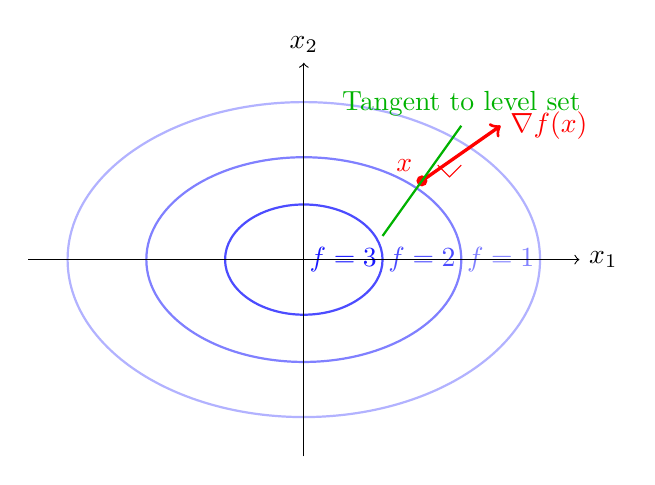
\begin{tikzpicture}[scale=1.0]
    % Contour plot (ellipses)
    \draw[blue!30, thick] (0,0) ellipse (3 and 2);
    \draw[blue!50, thick] (0,0) ellipse (2 and 1.3);
    \draw[blue!70, thick] (0,0) ellipse (1 and 0.7);
    
    % Level set labels
    \node[blue!50] at (2.5, 0) {$f = 1$};
    \node[blue!70] at (1.5, 0) {$f = 2$};
    \node[blue!90] at (0.5, 0) {$f = 3$};
    
    % Point on surface
    \fill[red] (1.5, 1) circle (2pt);
    \node[red, above left] at (1.5, 1) {$\vect{x}$};
    
    % Gradient vector (perpendicular to level set)
    \draw[->, red, very thick] (1.5, 1) -- (2.5, 1.7);
    \node[red, right] at (2.5, 1.7) {$\nabla f(\vect{x})$};
    
    % Tangent to level set
    \draw[green!70!black, thick] (1, 0.3) -- (2, 1.7);
    \node[green!70!black, above] at (2, 1.7) {Tangent to level set};
    
    % Right angle
    \draw[red, thin] (1.7, 1.2) -- (1.85, 1.05) -- (2, 1.2);
    
    \draw[->] (-3.5,0) -- (3.5,0) node[right] {$x_1$};
    \draw[->] (0,-2.5) -- (0,2.5) node[above] {$x_2$};
\end{tikzpicture}
\end{center}

Key insight: The gradient $\nabla f$ is \textit{perpendicular} to the level set (contour line). It points ``uphill'' toward higher function values.
\end{visualbox}

\begin{theorem}[Gradient Direction Property]
The gradient $\nabla f(\vect{x})$ points in the direction of maximum rate of increase of $f$ at $\vect{x}$.

Conversely, $-\nabla f(\vect{x})$ points in the direction of maximum rate of decrease (steepest descent).

\textbf{Proof sketch:} The directional derivative (rate of change in direction $\vect{v}$) is:

\begin{equation}
    D_{\vect{v}} f = \nabla f \cdot \vect{v} = \|\nabla f\| \|\vect{v}\| \cos \theta
\end{equation}

This is maximized when $\cos \theta = 1$, i.e., $\vect{v}$ is parallel to $\nabla f$.
\end{theorem}

\section{Directional Derivatives}

\begin{definition}[Directional Derivative]
The rate of change of $f$ at $\vect{x}$ in direction $\vect{v}$ (unit vector) is:

\begin{equation}
    D_{\vect{v}} f(\vect{x}) = \nabla f(\vect{x}) \cdot \vect{v} = \sum_{i=1}^n \frac{\partial f}{\partial x_i} v_i
\end{equation}

\textbf{Special cases:}
\begin{itemize}
    \item Direction $\vect{e}_i$ (standard basis): $D_{\vect{e}_i} f = \frac{\partial f}{\partial x_i}$
    \item Direction $\nabla f / \|\nabla f\|$: Maximum rate of increase
    \item Direction $-\nabla f / \|\nabla f\|$: Maximum rate of decrease
\end{itemize}
\end{definition}

\begin{example}[Directional Derivative]
For $f(x, y) = x^2 + y^2$ at point $(1, 0)$ in direction $\vect{v} = \frac{1}{\sqrt{2}}(1, 1)$:

\begin{equation}
    \nabla f(1, 0) = \begin{bmatrix} 2x \\ 2y \end{bmatrix}\bigg|_{(1,0)} = \begin{bmatrix} 2 \\ 0 \end{bmatrix}
\end{equation}

\begin{equation}
    D_{\vect{v}} f = \begin{bmatrix} 2 \\ 0 \end{bmatrix} \cdot \frac{1}{\sqrt{2}}\begin{bmatrix} 1 \\ 1 \end{bmatrix} = \frac{2}{\sqrt{2}} = \sqrt{2}
\end{equation}

Interpretation: Moving northeast from $(1, 0)$, $f$ increases at rate $\sqrt{2}$ per unit distance.
\end{example}

\section{The Jacobian: Derivatives of Vector Functions}

\subsection{Motivation}

Many ML functions map vectors to vectors:
\begin{itemize}
    \item Neural network layer: $\vect{h} = \vect{Wx} + \vect{b}$
    \item Softmax function: $\mathbb{R}^n \to \mathbb{R}^n$
    \item Coordinate transformations in robotics
\end{itemize}

For $\vect{f}: \mathbb{R}^n \to \mathbb{R}^m$, we need a matrix of derivatives.

\begin{seanbox}{6.3}
\textbf{Jacobian Matrix:}

For $\vect{f}(\vect{x}) = (f_1(\vect{x}), \ldots, f_m(\vect{x}))^\top$, the \textbf{Jacobian} is:

\begin{equation}
    \vect{J}_{\vect{f}}(\vect{x}) = \frac{\partial \vect{f}}{\partial \vect{x}} = \begin{bmatrix}
        \frac{\partial f_1}{\partial x_1} & \cdots & \frac{\partial f_1}{\partial x_n} \\
        \vdots & \ddots & \vdots \\
        \frac{\partial f_m}{\partial x_1} & \cdots & \frac{\partial f_m}{\partial x_n}
    \end{bmatrix} \in \mathbb{R}^{m \times n}
\end{equation}

\textbf{Row $i$}: Gradient of $f_i$ (how output $i$ changes with inputs)

\textbf{Column $j$}: Partial derivatives with respect to $x_j$ (how all outputs change with input $j$)

\textbf{Special case}: When $m = 1$, Jacobian is just the gradient (row vector).
\end{seanbox}

\begin{example}[Jacobian of Affine Transformation]
For $\vect{f}(\vect{x}) = \vect{Ax} + \vect{b}$ where $\vect{A} \in \mathbb{R}^{m \times n}$:

\begin{equation}
    \vect{J}_{\vect{f}} = \vect{A}
\end{equation}

(The linear part doesn't depend on $\vect{x}$; $\vect{b}$ disappears in derivative.)
\end{example}

\begin{example}[Jacobian of Elementwise Function]
For $\vect{f}(\vect{x}) = (\sigma(x_1), \ldots, \sigma(x_n))^\top$ where $\sigma$ is sigmoid:

\begin{equation}
    \vect{J}_{\vect{f}} = \text{diag}(\sigma'(x_1), \ldots, \sigma'(x_n))
\end{equation}

(Diagonal matrix because each output depends only on corresponding input.)
\end{example}

\subsection{The Chain Rule for Vector Functions}

\begin{theorem}[Multivariable Chain Rule]
If $\vect{f}: \mathbb{R}^n \to \mathbb{R}^m$ and $\vect{g}: \mathbb{R}^m \to \mathbb{R}^p$, then:

\begin{equation}
    \vect{J}_{\vect{g} \circ \vect{f}}(\vect{x}) = \vect{J}_{\vect{g}}(\vect{f}(\vect{x})) \cdot \vect{J}_{\vect{f}}(\vect{x})
\end{equation}

In dimensions: $(p \times n) = (p \times m) \cdot (m \times n)$

\textbf{This is backpropagation!}
\end{theorem}

\begin{philobox}
\textbf{The Chain Rule as Composition of Local Linearizations}

The chain rule states that the derivative of a composition is the product of derivatives. Philosophically, this embodies the idea that:

\begin{center}
\itshape
``To understand a complex transformation, compose the local linear approximations.''
\end{center}

Each Jacobian $\vect{J}_{\vect{f}}(\vect{x})$ is the \textit{best linear approximation} to $\vect{f}$ near $\vect{x}$:

\begin{equation}
    \vect{f}(\vect{x} + \Delta \vect{x}) \approx \vect{f}(\vect{x}) + \vect{J}_{\vect{f}}(\vect{x}) \Delta \vect{x}
\end{equation}

Composing functions is equivalent to composing their local linearizations (matrix multiplication). This is why deep learning works: each layer is locally linear, and the chain rule propagates gradients backward through these local approximations.

The notation $\vect{J}_{\vect{g} \circ \vect{f}} = \vect{J}_{\vect{g}} \cdot \vect{J}_{\vect{f}}$ is elegant: composition of functions becomes multiplication of matrices.
\end{philobox}

\section{The Hessian: Second Derivatives and Curvature}

\subsection{Motivation}

The gradient tells us the direction of steepest ascent. The \textbf{Hessian} tells us how the gradient itself is changing---i.e., the \textit{curvature} of the function.

\begin{seanbox}{6.4}
\textbf{Hessian Matrix:}

For $f: \mathbb{R}^n \to \mathbb{R}$, the \textbf{Hessian} is the matrix of second partial derivatives:

\begin{equation}
    \vect{H}_f(\vect{x}) = \begin{bmatrix}
        \frac{\partial^2 f}{\partial x_1^2} & \frac{\partial^2 f}{\partial x_1 \partial x_2} & \cdots & \frac{\partial^2 f}{\partial x_1 \partial x_n} \\
        \frac{\partial^2 f}{\partial x_2 \partial x_1} & \frac{\partial^2 f}{\partial x_2^2} & \cdots & \frac{\partial^2 f}{\partial x_2 \partial x_n} \\
        \vdots & \vdots & \ddots & \vdots \\
        \frac{\partial^2 f}{\partial x_n \partial x_1} & \frac{\partial^2 f}{\partial x_n \partial x_2} & \cdots & \frac{\partial^2 f}{\partial x_n^2}
    \end{bmatrix} \in \mathbb{R}^{n \times n}
\end{equation}

\textbf{Properties:}
\begin{itemize}
    \item Symmetric (if $f$ is $C^2$, by Schwarz's theorem)
    \item Entry $(i,j)$: How much $\frac{\partial f}{\partial x_i}$ changes with respect to $x_j$
    \item Diagonal: Second derivatives (how gradient component changes with itself)
    \item Off-diagonal: Mixed partials (interaction effects)
\end{itemize}
\end{seanbox}

\subsection{Characterizing Critical Points}

\begin{theorem}[Second Derivative Test]
At a critical point $\vect{x}^*$ (where $\nabla f(\vect{x}^*) = \vect{0}$):

\begin{itemize}
    \item If $\vect{H}_f(\vect{x}^*)$ is \textbf{positive definite} (all eigenvalues $> 0$): \\
    $\vect{x}^*$ is a \textbf{local minimum}
    
    \item If $\vect{H}_f(\vect{x}^*)$ is \textbf{negative definite} (all eigenvalues $< 0$): \\
    $\vect{x}^*$ is a \textbf{local maximum}
    
    \item If $\vect{H}_f(\vect{x}^*)$ has both positive and negative eigenvalues: \\
    $\vect{x}^*$ is a \textbf{saddle point}
    
    \item If $\vect{H}_f(\vect{x}^*)$ is indefinite (zero eigenvalues): \\
    Test is \textbf{inconclusive}
\end{itemize}
\end{theorem}

\begin{example}[Hessian of Quadratic Function]
For $f(x_1, x_2) = x_1^2 + 3x_1 x_2 + x_2^2$:

\begin{equation}
    \vect{H}_f = \begin{bmatrix} 2 & 3 \\ 3 & 2 \end{bmatrix}
\end{equation}

Eigenvalues: $\lambda_1 = 5, \lambda_2 = -1$ (one positive, one negative).

Therefore, $(0, 0)$ is a \textbf{saddle point}.
\end{example}

\begin{visualbox}
\textbf{Hessian Eigenvalues and Curvature:}

\begin{center}
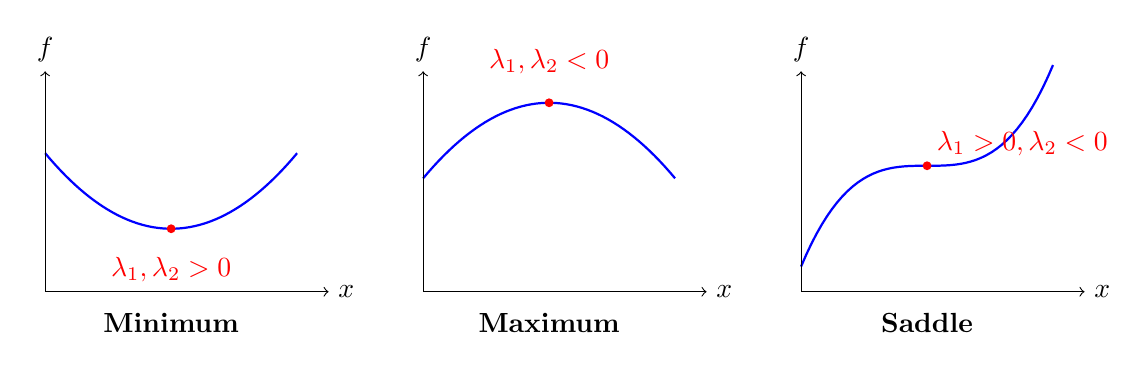
\begin{tikzpicture}[scale=0.8]
    % Local minimum (positive definite)
    \begin{scope}
        \node at (2, -0.5) {\textbf{Minimum}};
        \draw[blue, thick, domain=0:4, samples=50] plot (\x, {0.3*(\x-2)^2 + 1});
        \fill[red] (2, 1) circle (2pt);
        \node[red, below] at (2, 0.7) {$\lambda_1, \lambda_2 > 0$};
        \draw[->] (0,0) -- (4.5,0) node[right] {$x$};
        \draw[->] (0,0) -- (0,3.5) node[above] {$f$};
    \end{scope}
    
    % Local maximum (negative definite)
    \begin{scope}[xshift=6cm]
        \node at (2, -0.5) {\textbf{Maximum}};
        \draw[blue, thick, domain=0:4, samples=50] plot (\x, {-0.3*(\x-2)^2 + 3});
        \fill[red] (2, 3) circle (2pt);
        \node[red, above] at (2, 3.3) {$\lambda_1, \lambda_2 < 0$};
        \draw[->] (0,0) -- (4.5,0) node[right] {$x$};
        \draw[->] (0,0) -- (0,3.5) node[above] {$f$};
    \end{scope}
    
    % Saddle point (indefinite)
    \begin{scope}[xshift=12cm]
        \node at (2, -0.5) {\textbf{Saddle}};
        \draw[blue, thick, domain=0:4, samples=50] plot (\x, {0.2*(\x-2)^3 + 2});
        \fill[red] (2, 2) circle (2pt);
        \node[red, above right] at (2, 2) {$\lambda_1 > 0, \lambda_2 < 0$};
        \draw[->] (0,0) -- (4.5,0) node[right] {$x$};
        \draw[->] (0,0) -- (0,3.5) node[above] {$f$};
    \end{scope}
\end{tikzpicture}
\end{center}

The sign of Hessian eigenvalues determines whether a critical point is a minimum, maximum, or saddle.
\end{visualbox}

\section{Gradient Descent and Optimization}

\subsection{The Gradient Descent Algorithm}

\begin{seanbox}{6.5}
\textbf{Gradient Descent:}

To minimize $f(\vect{x})$, iteratively update:

\begin{equation}
    \vect{x}_{t+1} = \vect{x}_t - \alpha \nabla f(\vect{x}_t)
\end{equation}

where:
\begin{itemize}
    \item $\alpha > 0$ is the \textbf{learning rate} (step size)
    \item $\nabla f(\vect{x}_t)$ is the gradient at current point
    \item $-\nabla f$ points in direction of steepest descent
\end{itemize}

\textbf{Intuition:} Take a small step downhill, then recompute the gradient and repeat.

\textbf{Convergence:} Under convexity and Lipschitz conditions, converges to global minimum.
\end{seanbox}

\begin{codebox}
\textbf{Gradient Descent in Python:}

\begin{lstlisting}
import numpy as np

def gradient_descent(f, grad_f, x0, alpha=0.01, max_iter=1000, tol=1e-6):
    """
    Minimize function f using gradient descent.
    
    Args:
        f: Objective function
        grad_f: Gradient of f (returns vector)
        x0: Initial point
        alpha: Learning rate
        max_iter: Maximum iterations
        tol: Convergence tolerance
    
    Returns:
        x: Minimum point
        history: List of function values
    """
    x = x0.copy()
    history = [f(x)]
    
    for i in range(max_iter):
        grad = grad_f(x)
        x_new = x - alpha * grad
        
        # Check convergence
        if np.linalg.norm(x_new - x) < tol:
            print(f"Converged after {i+1} iterations")
            break
        
        x = x_new
        history.append(f(x))
    
    return x, history

# Example: Minimize f(x) = x^2 + y^2
def f(x):
    return x[0]**2 + x[1]**2

def grad_f(x):
    return np.array([2*x[0], 2*x[1]])

# Run gradient descent
x0 = np.array([5.0, 5.0])
x_min, history = gradient_descent(f, grad_f, x0, alpha=0.1)

print(f"Minimum at: {x_min}")
print(f"Function value: {f(x_min)}")

# Visualize convergence
import matplotlib.pyplot as plt
plt.plot(history)
plt.xlabel('Iteration')
plt.ylabel('Function Value')
plt.title('Gradient Descent Convergence')
plt.yscale('log')
plt.grid(True)
plt.show()
\end{lstlisting}
\end{codebox}

\subsection{Variants of Gradient Descent}

\begin{seanbox}{6.6}
\textbf{Stochastic Gradient Descent (SGD):}

For loss $L(\theta) = \frac{1}{m} \sum_{i=1}^m \ell(\theta; x^{(i)})$:

\textbf{Full-batch GD:}
\begin{equation}
    \theta_{t+1} = \theta_t - \alpha \nabla L(\theta_t) = \theta_t - \frac{\alpha}{m} \sum_{i=1}^m \nabla \ell(\theta_t; x^{(i)})
\end{equation}

\textbf{Stochastic GD:} Use single sample
\begin{equation}
    \theta_{t+1} = \theta_t - \alpha \nabla \ell(\theta_t; x^{(i_t)})
\end{equation}

\textbf{Mini-batch GD:} Use small batch $\mathcal{B}_t$
\begin{equation}
    \theta_{t+1} = \theta_t - \frac{\alpha}{|\mathcal{B}_t|} \sum_{i \in \mathcal{B}_t} \nabla \ell(\theta_t; x^{(i)})
\end{equation}

\textbf{Tradeoffs:}
\begin{itemize}
    \item Full-batch: Accurate but slow
    \item Stochastic: Fast but noisy (high variance)
    \item Mini-batch: Balance of speed and stability
\end{itemize}
\end{seanbox}

\begin{seanbox}{6.7}
\textbf{Advanced Optimizers:}

\textbf{Momentum:}
\begin{align}
    \vect{v}_{t+1} &= \beta \vect{v}_t + \nabla f(\vect{x}_t) \\
    \vect{x}_{t+1} &= \vect{x}_t - \alpha \vect{v}_{t+1}
\end{align}

(Accumulates gradient history, smooths updates)

\textbf{RMSprop:}
\begin{align}
    \vect{s}_{t+1} &= \beta \vect{s}_t + (1-\beta) (\nabla f)^2 \\
    \vect{x}_{t+1} &= \vect{x}_t - \frac{\alpha}{\sqrt{\vect{s}_{t+1}} + \epsilon} \nabla f
\end{align}

(Adapts learning rate per dimension)

\textbf{Adam:} Combines momentum + RMSprop
\begin{align}
    \vect{m}_{t+1} &= \beta_1 \vect{m}_t + (1-\beta_1) \nabla f \quad \text{(1st moment)} \\
    \vect{v}_{t+1} &= \beta_2 \vect{v}_t + (1-\beta_2) (\nabla f)^2 \quad \text{(2nd moment)} \\
    \hat{\vect{m}} &= \frac{\vect{m}_{t+1}}{1 - \beta_1^{t+1}}, \quad \hat{\vect{v}} = \frac{\vect{v}_{t+1}}{1 - \beta_2^{t+1}} \quad \text{(bias correction)} \\
    \vect{x}_{t+1} &= \vect{x}_t - \frac{\alpha \hat{\vect{m}}}{\sqrt{\hat{\vect{v}}} + \epsilon}
\end{align}

(Default choice in deep learning; typical: $\beta_1 = 0.9, \beta_2 = 0.999$)
\end{seanbox}

\section{Backpropagation: The Chain Rule in Action}

\subsection{Neural Network as Composed Functions}

A neural network is a composition:

\begin{equation}
    f(\vect{x}; \theta) = f_L \circ f_{L-1} \circ \cdots \circ f_1(\vect{x})
\end{equation}

where each layer $f_\ell$ is typically:

\begin{equation}
    f_\ell(\vect{h}_{\ell-1}) = \sigma(\vect{W}_\ell \vect{h}_{\ell-1} + \vect{b}_\ell)
\end{equation}

To train via gradient descent, we need $\frac{\partial L}{\partial \vect{W}_\ell}$ and $\frac{\partial L}{\partial \vect{b}_\ell}$ for all layers.

\begin{seanbox}{6.8}
\textbf{Backpropagation Algorithm:}

\textbf{Forward pass:} Compute activations layer by layer

\begin{align}
    \vect{h}_0 &= \vect{x} \\
    \vect{z}_\ell &= \vect{W}_\ell \vect{h}_{\ell-1} + \vect{b}_\ell \quad \text{(pre-activation)} \\
    \vect{h}_\ell &= \sigma(\vect{z}_\ell) \quad \text{(activation)} \\
    \hat{y} &= \vect{h}_L \quad \text{(output)}
\end{align}

\textbf{Backward pass:} Compute gradients using chain rule

\begin{align}
    \delta_L &= \frac{\partial L}{\partial \vect{h}_L} \quad \text{(output error)} \\
    \delta_\ell &= (\vect{W}_{\ell+1}^\top \delta_{\ell+1}) \odot \sigma'(\vect{z}_\ell) \quad \text{(backpropagate error)} \\
    \frac{\partial L}{\partial \vect{W}_\ell} &= \delta_\ell \vect{h}_{\ell-1}^\top \quad \text{(weight gradient)} \\
    \frac{\partial L}{\partial \vect{b}_\ell} &= \delta_\ell \quad \text{(bias gradient)}
\end{align}

where $\odot$ is elementwise multiplication.

\textbf{Key insight:} The chain rule factorizes as:

\begin{equation}
    \frac{\partial L}{\partial \vect{W}_\ell} = \frac{\partial L}{\partial \vect{h}_L} \cdot \frac{\partial \vect{h}_L}{\partial \vect{h}_{L-1}} \cdots \frac{\partial \vect{h}_{\ell+1}}{\partial \vect{h}_\ell} \cdot \frac{\partial \vect{h}_\ell}{\partial \vect{W}_\ell}
\end{equation}

We compute this product \textit{right to left} (backward), reusing intermediate results.
\end{seanbox}

\begin{philobox}
\textbf{Backpropagation as Automatic Differentiation}

Backpropagation is not a heuristic---it's the \textit{automatic} application of the chain rule to computational graphs.

\textbf{Computational graph}: Directed acyclic graph where:
\begin{itemize}
    \item Nodes = variables or operations
    \item Edges = dependencies
\end{itemize}

\textbf{Forward mode}: Compute function values (data flows forward)

\textbf{Reverse mode (backprop)}: Compute gradients (errors flow backward)

The notation $\delta_\ell = (\vect{W}_{\ell+1}^\top \delta_{\ell+1}) \odot \sigma'(\vect{z}_\ell)$ encodes:
\begin{enumerate}
    \item Receive error signal from layer above: $\delta_{\ell+1}$
    \item Multiply by Jacobian of layer $\ell+1$: $\vect{W}_{\ell+1}^\top$
    \item Modulate by local derivative: $\sigma'(\vect{z}_\ell)$
\end{enumerate}

This is the chain rule in matrix form. Modern frameworks (PyTorch, TensorFlow) implement this automatically via autodiff.
\end{philobox}

\subsection{Example: Two-Layer Network}

\begin{codebox}
\textbf{Manual Backpropagation (Pedagogical):}

\begin{lstlisting}
import numpy as np

def sigmoid(z):
    return 1 / (1 + np.exp(-z))

def sigmoid_derivative(z):
    s = sigmoid(z)
    return s * (1 - s)

# Network architecture: 2 -> 3 -> 1
np.random.seed(42)
W1 = np.random.randn(3, 2) * 0.1
b1 = np.zeros((3, 1))
W2 = np.random.randn(1, 3) * 0.1
b2 = np.zeros((1, 1))

# Forward pass
x = np.array([[1.0], [0.5]])
y_true = np.array([[1.0]])

# Layer 1
z1 = W1 @ x + b1
h1 = sigmoid(z1)

# Layer 2
z2 = W2 @ h1 + b2
h2 = sigmoid(z2)
y_pred = h2

# Loss (MSE)
loss = 0.5 * (y_pred - y_true)**2

# Backward pass
# Output layer
dL_dy = (y_pred - y_true)  # Derivative of loss
dy_dz2 = sigmoid_derivative(z2)
delta2 = dL_dy * dy_dz2

dL_dW2 = delta2 @ h1.T
dL_db2 = delta2

# Hidden layer
dL_dh1 = W2.T @ delta2
dh1_dz1 = sigmoid_derivative(z1)
delta1 = dL_dh1 * dh1_dz1

dL_dW1 = delta1 @ x.T
dL_db1 = delta1

print(f"Loss: {loss.item():.4f}")
print(f"dL/dW2:\n{dL_dW2}")
print(f"dL/dW1:\n{dL_dW1}")

# Gradient descent update
alpha = 0.1
W2 -= alpha * dL_dW2
b2 -= alpha * dL_db2
W1 -= alpha * dL_dW1
b1 -= alpha * dL_db1
\end{lstlisting}
\end{codebox}

\section{Applications in Machine Learning}

\subsection{Linear Regression: Closed-Form Solution}

\begin{example}[Normal Equations]
For linear regression $\min_{\vect{w}} \|\vect{Xw} - \vect{y}\|^2$:

Set gradient to zero:
\begin{align}
    \nabla_{\vect{w}} (\vect{Xw} - \vect{y})^\top (\vect{Xw} - \vect{y}) &= \vect{0} \\
    2\vect{X}^\top(\vect{Xw} - \vect{y}) &= \vect{0} \\
    \vect{X}^\top \vect{Xw} &= \vect{X}^\top \vect{y} \\
    \vect{w}^* &= (\vect{X}^\top \vect{X})^{-1} \vect{X}^\top \vect{y}
\end{align}

This is the \textbf{normal equation}---a direct application of setting gradient to zero.
\end{example}

\subsection{Logistic Regression: Iterative Solution}

\begin{example}[Gradient Descent for Logistic Regression]
Loss: $L(\vect{w}) = -\sum_{i=1}^m [y^{(i)} \log \hat{y}^{(i)} + (1-y^{(i)}) \log(1-\hat{y}^{(i)})]$

where $\hat{y}^{(i)} = \sigma(\vect{w}^\top \vect{x}^{(i)})$.

Gradient:
\begin{equation}
    \nabla_{\vect{w}} L = \sum_{i=1}^m (\hat{y}^{(i)} - y^{(i)}) \vect{x}^{(i)}
\end{equation}

Update:
\begin{equation}
    \vect{w}_{t+1} = \vect{w}_t - \alpha \nabla_{\vect{w}} L
\end{equation}

No closed-form solution, so we use iterative gradient descent.
\end{example}

\section{Practical Considerations}

\subsection{Numerical Gradient Checking}

To verify analytical gradients, use \textbf{finite differences}:

\begin{equation}
    \frac{\partial f}{\partial x_i} \approx \frac{f(x + \epsilon e_i) - f(x - \epsilon e_i)}{2\epsilon}
\end{equation}

where $e_i$ is the $i$-th standard basis vector, $\epsilon \approx 10^{-4}$.

\begin{codebox}
\textbf{Gradient Checking:}

\begin{lstlisting}
def numerical_gradient(f, x, epsilon=1e-4):
    """
    Compute gradient numerically using finite differences.
    """
    grad = np.zeros_like(x)
    for i in range(len(x)):
        x_plus = x.copy()
        x_plus[i] += epsilon
        x_minus = x.copy()
        x_minus[i] -= epsilon
        grad[i] = (f(x_plus) - f(x_minus)) / (2 * epsilon)
    return grad

# Example: Check gradient of f(x) = x^T A x
def f(x):
    A = np.array([[2, 1], [1, 3]])
    return x @ A @ x

def grad_f(x):
    A = np.array([[2, 1], [1, 3]])
    return 2 * A @ x

x = np.array([1.0, 2.0])
grad_analytical = grad_f(x)
grad_numerical = numerical_gradient(f, x)

print("Analytical gradient:", grad_analytical)
print("Numerical gradient:", grad_numerical)
print("Difference:", np.linalg.norm(grad_analytical - grad_numerical))
\end{lstlisting}
\end{codebox}

\subsection{Vanishing and Exploding Gradients}

In deep networks, gradients can vanish or explode during backpropagation.

\begin{remark}[Gradient Pathologies]
Consider $L$ layers with weight matrices $\vect{W}_\ell$:

\begin{equation}
    \frac{\partial L}{\partial \vect{W}_1} \propto \prod_{\ell=2}^L \vect{W}_\ell \sigma'(\vect{z}_\ell)
\end{equation}

\textbf{Vanishing:} If $\|\vect{W}_\ell\| < 1$ and $|\sigma'| < 1$, product $\to 0$ exponentially.

\textbf{Exploding:} If $\|\vect{W}_\ell\| > 1$, product $\to \infty$ exponentially.

\textbf{Solutions:}
\begin{itemize}
    \item Careful weight initialization (Xavier, He)
    \item Activation functions (ReLU instead of sigmoid)
    \item Batch normalization
    \item Residual connections (skip connections)
    \item Gradient clipping
\end{itemize}
\end{remark}

\section{Reflective Exercises}

\begin{exercise}[Computing Gradients]
Compute the gradient of $f(x, y) = e^{x^2 + y^2}$ at $(1, 0)$.
\end{exercise}

\begin{exercise}[Hessian Analysis]
For $f(x, y) = x^3 - 3xy^2$, find all critical points and classify them using the Hessian.
\end{exercise}

\begin{exercise}[Gradient Descent Convergence]
Implement gradient descent for $f(x) = 0.1x^2$ and $g(x) = 100x^2$. Compare convergence rates. What does this reveal about the importance of learning rate?
\end{exercise}

\begin{exercise}[Chain Rule Practice]
For $f(x) = \log(\exp(x^2) + 1)$, compute $f'(x)$ using the chain rule.
\end{exercise}

\begin{exercise}[Jacobian Calculation]
For $\vect{f}(x, y) = (x^2 + y^2, xy)^\top$, compute the Jacobian matrix.
\end{exercise}

\begin{exercise}[Coding: Implement Backpropagation]
Write a three-layer neural network from scratch (no frameworks) and implement manual backpropagation. Verify gradients using numerical differentiation.
\end{exercise}

\begin{exercise}[Philosophical: Gradients and Knowledge]
The gradient points in the direction of steepest ascent. In what sense does "following the negative gradient" constitute "learning"? How does this relate to the philosophical problem of induction?
\end{exercise}

\section{Connections to Other Parts}

\subsection{To Part I (Linear Algebra)}
\begin{itemize}
    \item Jacobian matrix connects linear algebra with calculus
    \item Eigenvalues of Hessian determine curvature
    \item Matrix multiplication appears in chain rule
\end{itemize}

\subsection{To Part II (Statistics)}
\begin{itemize}
    \item Maximum likelihood estimation uses gradient descent
    \item Fisher information matrix is related to Hessian
    \item Stochastic gradient descent connects to sampling theory
\end{itemize}

\subsection{To Part III (Neural Networks)}
\begin{itemize}
    \item Backpropagation is the chain rule applied to neural nets
    \item Activation functions must be differentiable
    \item Gradient clipping prevents training instability
\end{itemize}

\subsection{To Part IV (Clustering)}
\begin{itemize}
    \item K-means uses gradients implicitly in centroid updates
    \item GMM parameter estimation uses EM (derivative-free optimization)
\end{itemize}

\subsection{To Part V (Reinforcement Learning)}
\begin{itemize}
    \item Policy gradients optimize expected reward
    \item Actor-critic methods use gradients for both actor and critic
    \item TD error is a form of gradient signal
\end{itemize}

\section{Conclusion: Calculus as the Language of Optimization}

Vector calculus is the \textbf{foundation of modern machine learning}. Every training algorithm, from simple linear regression to complex deep reinforcement learning, relies on computing and following gradients.

\textbf{Key Takeaways:}

\begin{enumerate}
    \item \textbf{Gradient} = Direction of steepest ascent (negative gradient = descent)
    \item \textbf{Jacobian} = Matrix of partial derivatives for vector functions
    \item \textbf{Hessian} = Matrix of second derivatives (curvature information)
    \item \textbf{Chain rule} = Composition of functions $\to$ product of derivatives
    \item \textbf{Backpropagation} = Efficient computation of gradients via chain rule
    \item \textbf{Gradient descent} = Iterative optimization by following negative gradient
\end{enumerate}

\begin{center}
\itshape
``Without calculus, machine learning would be blind—unable to see \\
which direction leads to better predictions, which parameters \\
improve performance, which path descends toward the optimum.''
\end{center}

\vspace{1cm}

As you proceed through more advanced topics, remember that underneath every sophisticated algorithm lies this fundamental idea: \textit{compute the gradient, take a step in that direction, repeat}. Mastering vector calculus means mastering the language in which machines learn.

\clearpage
